\documentclass{article}\usepackage[]{graphicx}\usepackage[]{color}
%% maxwidth is the original width if it is less than linewidth
%% otherwise use linewidth (to make sure the graphics do not exceed the margin)
\makeatletter
\def\maxwidth{ %
  \ifdim\Gin@nat@width>\linewidth
    \linewidth
  \else
    \Gin@nat@width
  \fi
}
\makeatother

\definecolor{fgcolor}{rgb}{0.345, 0.345, 0.345}
\newcommand{\hlnum}[1]{\textcolor[rgb]{0.686,0.059,0.569}{#1}}%
\newcommand{\hlstr}[1]{\textcolor[rgb]{0.192,0.494,0.8}{#1}}%
\newcommand{\hlcom}[1]{\textcolor[rgb]{0.678,0.584,0.686}{\textit{#1}}}%
\newcommand{\hlopt}[1]{\textcolor[rgb]{0,0,0}{#1}}%
\newcommand{\hlstd}[1]{\textcolor[rgb]{0.345,0.345,0.345}{#1}}%
\newcommand{\hlkwa}[1]{\textcolor[rgb]{0.161,0.373,0.58}{\textbf{#1}}}%
\newcommand{\hlkwb}[1]{\textcolor[rgb]{0.69,0.353,0.396}{#1}}%
\newcommand{\hlkwc}[1]{\textcolor[rgb]{0.333,0.667,0.333}{#1}}%
\newcommand{\hlkwd}[1]{\textcolor[rgb]{0.737,0.353,0.396}{\textbf{#1}}}%

\usepackage{framed}
\makeatletter
\newenvironment{kframe}{%
 \def\at@end@of@kframe{}%
 \ifinner\ifhmode%
  \def\at@end@of@kframe{\end{minipage}}%
  \begin{minipage}{\columnwidth}%
 \fi\fi%
 \def\FrameCommand##1{\hskip\@totalleftmargin \hskip-\fboxsep
 \colorbox{shadecolor}{##1}\hskip-\fboxsep
     % There is no \\@totalrightmargin, so:
     \hskip-\linewidth \hskip-\@totalleftmargin \hskip\columnwidth}%
 \MakeFramed {\advance\hsize-\width
   \@totalleftmargin\z@ \linewidth\hsize
   \@setminipage}}%
 {\par\unskip\endMakeFramed%
 \at@end@of@kframe}
\makeatother

\definecolor{shadecolor}{rgb}{.97, .97, .97}
\definecolor{messagecolor}{rgb}{0, 0, 0}
\definecolor{warningcolor}{rgb}{1, 0, 1}
\definecolor{errorcolor}{rgb}{1, 0, 0}
\newenvironment{knitrout}{}{} % an empty environment to be redefined in TeX

\usepackage{alltt}
\usepackage{amsmath,amsfonts,bm,fullpage,multirow,animate,subcaption,graphicx,caption}
\usepackage{natbib,tikz}
\bibliographystyle{abbrvnat}
\DeclareMathOperator*{\argmax}{arg\,max}
\newcommand{\ProjMean}{{\widehat{\bm S}_{E}}}
\newcommand{\ProjMedian}{{\widetilde{\bm S}_{E}}}
\newcommand{\GeomMean}{{\widehat{\bm S}_{R}}}
\newcommand{\GeomMedian}{{\widetilde{\bm S}_{R}}}
\newcommand{\HuberMean}{{\widehat{\bm S}_H}}
\newcommand{\WeightMean}{{\widehat{\bm S}_W}}
\newcommand{\TrimMean}{{\widehat{\bm S}_T}}
\newcommand{\WinzMean}{{\widehat{\bm S}_Z}}
\newcommand{\R}{{\mathbb{R}}}
\newcommand{\qest}{{\hat{\bm q}}}
\newcommand{\Sest}{{\widehat{\bm S}}}
\newcommand{\red}[1]{{\color{red} #1}}
\IfFileExists{upquote.sty}{\usepackage{upquote}}{}
\begin{document}

\begin{center}
\Large{\bf Extreme Observation Identification and Accommodation in the Rotation Group $SO(3)$}
\end{center}
\begin{abstract}
Similar to data on the circle and sphere, random matrices in the rotation group SO(3) lie in a bounded space and are often highly concentrated.  As such, data analysis techniques that identify and accommodate for extreme observations in SO(3) have received little attention.  With the increased use of tools that result in observations in SO(3), e.g.~Electron Backscatter Diffraction, extreme observations have become increasingly common though their treatment is still rudimentary.  In this paper we propose a definition of outlier in a variety of contexts.  Once an extreme observation has been identified, we propose a modified multi-dimensional Huber estimator as well as trimmed and winsorized means in SO(3) that are resistant to extreme observations with minimal cost to bias and standard error.  We demonstrate the behavior of these estimators relative to those that already exist in a simulation study and data example.
\end{abstract}

\section{Introduction}\label{sec:intro}
This is a summary of the material related to robustness for $SO(3)$ data.  A detailed account of outlier detection for circular and spherical data can be found in ``Outliers.pdf."  More detail on the robustified $L_2$ estimator can be found in ``TrimMeanSimulation.pdf."



 
\section{Outlier Detection}\label{sec:outliers}
 
I have not found a formal discussion or definition of outliers for rotations. \cite{fletcher2008} use the term `outlier' a lot in connection with rotation data, but it is never defined.  For their simulation study they simulate some data from a distribution with one central direction $\bm S$, then simulate the rest of the data from the same distribution with mean rotated through $90^\circ$.

Two of the most promising leads on outlier detection in $SO(3)$ is a generalization of \cite{collett1980} $C$-statistic and the $H_n$ statistic of (originally) \cite{best1986} and later \cite{figueiredo2005}.  The Collett's $C$-statistic boils down to how much your estimate of center moves when a particular observation is removed.  The $H_n$-statistic is based on axial data (like quaternions) and quantifies how far from the bulk of the data a particular observation lies.  More details on these statistics are below.  Since $H_n$ is based on the quaternion representation of rotation I will use quaternions throughout. 

For a sample of rotations $\bm q_1,\dots,\bm q_n$ let $\qest$ denote the estimated center.  Define the rotation analog of the Collett's $C$-statistic as 
\begin{equation}\label{eqn:Ci}
C_i=d_E(\qest,\hat{\bm q}^{(i)})=\sqrt{8[1-(\qest^\top\qest^{(i)})]}
\end{equation}
where $d_E$ is the Euclidean distance and $\qest^{(i)}$ is the estimated central direction when the $i$th observation is deleted.  

A special type of spherical data is axial data, that is $\bm X$ is said to come from an axial population if $\bm X_i$ and $-\bm X_i$ have the same distribution for all $i$.  Quaternions are one example of axial data.  Let $\bm Q$ denote the $n\times 4$ matrix with rows $\bm q_i$ and define $\bm T=\bm Q^\top\bm Q=\sum_{i=1}^n\bm q_i\bm q_i^\top$.  Further let $\hat\tau_1\leq\hat\tau_2\leq\hat\tau_3\leq\hat\tau_4$ denote the ordered eigenvalues of $\bm T_n$.  Similarly let $\bm T_{i}$ denote the matrix $\bm T$ with the $i$th observation deleted $\bm T_i=\bm T-\bm q_i\bm q_i^\top$, which has ordered eigenvalues $\hat\tau_{1,i}\leq\hat\tau_{2,i}\leq\hat\tau_{3,i}\leq\hat\tau_{4,i}$.  Define the statistic
\begin{equation}\label{eqn:Hj}
H_i=(n-2)\frac{1+\hat\tau_{4,i}-\hat\tau_4}{n-1-\hat\tau_{4,i}}.
\end{equation}
Under certain distribution assumptions on $\bm q_i$  $H_i$ has a limiting $F_{3,3(n-2)}$ distribution.  In general, large values of $H_i$ indicate the $i$th observation is far from the bulk of the data.

Another note on \eqref{eqn:Hj} is that for quaternion data the projected mean is the largest eigenvector associated with the largest eigenvalue of $\bm T$.  That is, the projected mean is the eigenvector associated with $\hat\tau_4$.  This makes me think that we should be able to express $H_i$ as a function of $C_i$ when $\qest=\hat{\bm q}_2$, though I have not been able to do this yet.  Next I explore this relationship for the extrinsic and intrinsic $L_2$ estimators on $SO(3)$. 

%There appears to be a connection between the statistic $H_n$ and Collett's $C$ statistic.  The $H_n$ statistic is a function of the difference in the largest eigenvalue of the matrix $T=\sum_{i=1}^n\bm q_i\bm q_i^\top$ when the $i$th observation has been removed.  Collett's $C$ statistic is the relative change in the mean resultant length when the $i$th observation has been removed.   The statistics $H_n$ and $C$ can be translated to rotation data most easily when we consider the quaternion representation.  This is because the projected mean in the quaternion case is the eigenvector associated with the largest eigenvalue of $T$.  

Figures \ref{fig:HnC} and \ref{fig:HnCGeom} illustrate the relationship between the $H_i$- and $C_i$-statistics for the projected and geometric means, respectively, in a concentrated data set (left) and a diffuse data set (right).  Both show a strong relationship between $C_i$ and $H_i$.  The color of each dot is determined by the distance each point is from the estimated center, $d_R(\bm R_i,\Sest)$ for the projected and geometric means.

\begin{figure}
\centering
\begin{subfigure}[b]{0.45\textwidth}
        \includegraphics[width=\textwidth]{Figure/HnCConcentrated}
        \caption{$\kappa=50$}
\end{subfigure}
\begin{subfigure}[b]{0.45\textwidth}
        \includegraphics[width=\textwidth]{Figure/HnCDiffuse}
        \caption{$\kappa=1$}
        \label{fig:HnDiff}
\end{subfigure}
\caption{The $H_i$ and $C_i$ statistics for a sample $n=25$ from the Cayley distribution with $\kappa=50$ (left) and $\kappa=1$ (right).  The points are colored based on each observations distance from the projected mean $\hat r_i=d_R(\bm R_i,\ProjMean$)}
\label{fig:HnC}
\end{figure}

\begin{figure}
\centering
\begin{subfigure}[b]{0.45\textwidth}
        \includegraphics[width=\textwidth]{Figure/HnCConcentratedGeometric}
        \caption{$\kappa=50$}
\end{subfigure}
\begin{subfigure}[b]{0.45\textwidth}
        \includegraphics[width=\textwidth]{Figure/HnCDiffuseGeometric}
        \caption{$\kappa=1$}
        \label{fig:HnDiffGeom}
\end{subfigure}
\caption{The $H_i$ and $C_i$ statistics for a sample from $n=25$ the Cayley distribution with $\kappa=50$ (left) and $\kappa=1$ (right).  The points are colored based on each observations distance from the geometric mean $\hat r_i=d_R(\bm R_i,\GeomMean$)}
\label{fig:HnCGeom}
\end{figure}

From Figure \ref{fig:HnDiff} it appears that the $C_i$ statistic based on the projected mean cannot distinguish between observations that are on the extremes of the spectrum, i.e.~are very close to the estimated center or a $90^\circ$ rotation away.  More specifically, $C$ is maximized for observations that are roughly $\pi/2$ radians away from the estimated central direction $\ProjMean$, while observations near or $\pi$ radians away from the estimated center have the same $C$ value.  %This same behavior is exhibited by the influence function.  From \eqref{eqn:IF}, the influence function of the projected mean is $IF(\bm R_i,F)\propto\sin(r_i)\bm U_i$ which is maximized (ignoring $\bm U_i$) at $r_i=\pi/2$ and is the same from $r_i=0$ or $r_i=\pi$.
The $H_n$ statistic, however, is closely related to the rotational distance between each observation and the estimated center $\ProjMean$.  I can show empirically that for $\bm R_i$ satisfying $d_R(\bm R_i,\ProjMean)=\pi/2$ both maximizes $C_i$ and $H_i=1$, but this would be nice to prove. 

From Figure \ref{fig:HnDiffGeom}, however, it is clear the $C_i$ statistic based on the geometric mean is linearly related to the $H_i$ statistic.  Therefore the geometric mean is influenced by observations away from the estimated center in a linear way, not a sinusoidal one.  The influence function for the geometric mean has not been determined yet, but based on these results, it will be proportional to $r_i$ and not $\sin(r_i)$.  This could be an argument for the intrinsic approach and against the extrinsic approach.


The question as to which statistic is appropriate comes down to: why do you care?  Large $C$ statistic (and also influence function) values will determine which observation will have the largest impact on the projected mean estimate of center.  The $H_n$ statistic will tell you which observation is most unlike the others, but not necessarily the one that will impact estimation.

\section{Influence Functions}\label{sec:ifs}

The \emph{influence function} of an estimator quantifies the change in that estimator when one sample point is changed.  In the regions paper we proved the influence function of the projected mean $\ProjMean$ based on a sample of directionally symmetric rotations $\bm R_i=\exp[\bm \Phi(r_i\bm U_i)]$ with central orientation $\bm S$ to be
\begin{equation}\label{eqn:IF}
\text{IF}(\bm R_i,F)=\frac{1}{d}\sin(r_i)\bm U_i
\end{equation}
where $d=[1+2E\cos(r_i)]/3$ and $\bm R_i=\bm S\exp[\bm\Phi(r_i\bm U_i)]$.  Heuristically the $C_i$-statistic of Section \ref{sec:outliers} is an empirical influence function.  The influence function of the geometric mean is not readily available, but the results to come next indicate it is a linear function of $r_i$ and not a sinusoidal one.

The influence function of $\GeomMean$ is not available in it full form, but it has been derived up to a constant.  More specifically the influence function of $\GeomMean$ is
\[
\text{IF}_{2R}(\bm R_i,F)\propto\sin^{-1}\left[\sqrt{\frac{1-\cos(r_i)}{2}}\right]\bm U_i= r_i\bm U_i.
\]
In Figure \ref{fig:IFs} the influence functions for the two $L_2$ estimators are compared as a function of $r_i$.  The $\bm U_i$ term is ignored, because the assumption that $\bm U_i$ is uniformly distributed on the unit sphere will make that term wash out.
 
\begin{figure}
\begin{center}
\includegraphics[width=.7\textwidth]{Figure/IFComparison.pdf}
\end{center}\vspace{-1em}
\caption{A comparison of the unstandardized influence functions for the $L_2$ estimators according to the extrinsic (red) and intrinsic (blue) approaches.}
\label{fig:IFs}
\end{figure} 
 
 
Looking at this relationship another way, consider Figures \ref{fig:circular} and \ref{fig:sample}.  In Figure \ref{fig:circular1} a random sample on the circle is plotted along with the projected mean estimate of the central orientation.  In \ref{fig:circular2} an additional observation is added that is the projected mean rotated through 180$^\circ$.  It is clear that the additional point moves the arithmetic mean $\overline{\bm R}$ closer to the center of the circle in Figure \ref{fig:circular2}, but the projection of the arithmetic mean $\ProjMean$ to the surface of the circle is unchanged.

To illustrate this on $SO(3)$ consider Figure \ref{fig:samp1}, in which the $x$-axis of a random sample from the Cayley($\bm I_{3\times 3},50$) distribution is plotted with both $L_2$ estimators, $\ProjMean$ and $\GeomMean$.  In Figure \ref{fig:samp2} the exact same sample is plotted, with the addition of an observation that is a rotation of $\ProjMean$ through $\pi$ radians.  The additional observation is marked with an ``X".  In the figure (and numerically) there is no difference between the projected mean in these two samples.  The geometric mean, however, moves away from the true center $\bm I_{3\times 3}$ as one would expect given the additional observation on the other pole.




\begin{figure}[h]
\begin{subfigure}[h]{0.4\textwidth}
\centering
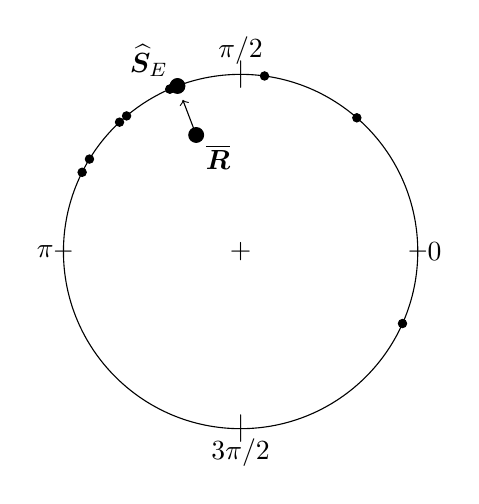
\begin{tikzpicture}[scale=.75]
    \draw (0,0) circle [radius=3];
    \node at (0,0) {$+$};
    \node at (-3,0) {$-$};\node [left] at(-3,0) {$\pi$};
    \node at (3,0) {$-$}; \node [right] at(3,0) {$0$};
    \node at (0,3) {$|$}; \node [above] at (0,3) {$\pi/2$};
    \node at (0,-3) {$|$}; \node [below] at (0,-3) {$3\pi/2$};
    \draw [fill] (-1.0250062,  2.819461) circle [radius=0.07]; %Sample 
    \draw [fill] (-1.2003083,  2.749411) circle [radius=0.07];
    \draw [fill] (0.4048608,  2.972556) circle [radius=0.07];
    \draw [fill] (-2.6833833,  1.341437) circle [radius=0.07];
    \draw [fill] (-2.0500236,  2.190298) circle [radius=0.07];
    \draw [fill] (2.7410225, -1.219342) circle [radius=0.07];
    \draw [fill] (-1.1894952,  2.754106) circle [radius=0.07];
    \draw [fill] (1.9681982,  2.264110) circle [radius=0.07];
    \draw [fill] (-2.5592776,  1.565279) circle [radius=0.07];
    \draw [fill] (-1.9309514,  2.295959) circle [radius=0.07];
    \draw [fill] (-0.7524364,  1.9733275) circle[radius=0.125]; %Arithmetic Mean
    \node [below right] at (-0.7524364,  1.9733275) {$\overline{\bm R}$};
    \draw [fill] (-1.068845,  2.803136) circle[radius=0.125]; %Projected Mean
    \node [above left] at (-1.068845,  2.803136) {$\widehat{\bm S}_E$};
    \draw [->] (-0.7524364,  1.9733275) -- (-0.9797747,  2.5695411);
\end{tikzpicture}
\caption{Original data, A}
\label{fig:circular1}
\end{subfigure}
\begin{subfigure}[h]{0.4\textwidth}
\centering
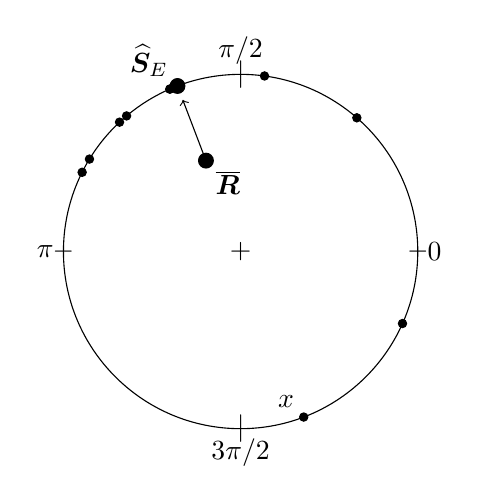
\begin{tikzpicture}[scale=.75]
    \draw (0,0) circle [radius=3];
    \node at (0,0) {$+$};
    \node at (-3,0) {$-$};\node [left] at(-3,0) {$\pi$};
    \node at (3,0) {$-$}; \node [right] at(3,0) {$0$};
    \node at (0,3) {$|$}; \node [above] at (0,3) {$\pi/2$};
    \node at (0,-3) {$|$}; \node [below] at (0,-3) {$3\pi/2$};
%     \node at (-1.0250062,  2.819461) {$\times$}; %Sample 
%     \node at (-1.2003083,  2.749411) {$\times$};
%     \node at (0.4048608,  2.972556) {$\times$};
%     \node at (-2.6833833,  1.341437) {$\times$};
%     \node at (-2.0500236,  2.190298) {$\times$};
%     \node at (2.7410225, -1.219342) {$\times$};
%     \node at (-1.1894952,  2.754106) {$\times$};
%     \node at (1.9681982,  2.264110) {$\times$};
%     \node at (-2.5592776,  1.565279) {$\times$};
%     \node at (-1.9309514,  2.295959) {$\times$};
    \draw [fill] (-1.0250062,  2.819461) circle [radius=0.07]; %Sample 
    \draw [fill] (-1.2003083,  2.749411) circle [radius=0.07];
    \draw [fill] (0.4048608,  2.972556) circle [radius=0.07];
    \draw [fill] (-2.6833833,  1.341437) circle [radius=0.07];
    \draw [fill] (-2.0500236,  2.190298) circle [radius=0.07];
    \draw [fill] (2.7410225, -1.219342) circle [radius=0.07];
    \draw [fill] (-1.1894952,  2.754106) circle [radius=0.07];
    \draw [fill] (1.9681982,  2.264110) circle [radius=0.07];
    \draw [fill] (-2.5592776,  1.565279) circle [radius=0.07];
    \draw [fill] (-1.9309514,  2.295959) circle [radius=0.07];
    \draw [fill] (-0.5868654,  1.5391035) circle[radius=0.125]; %New Arithmetic Mean
    \node [below right] at (-0.5868654,  1.5391035) {$\overline{\bm R}$};
    \draw [fill] (-1.068845,  2.803136) circle[radius=0.125]; %Projected Mean
    \node [above left] at (-1.068845,  2.803136) {$\widehat{\bm S}_E$};
    \draw [->] (-0.5868654,  1.5391035) -- (-0.9797747,  2.5695411);
    \draw [fill] (1.068845, -2.803136) circle [radius=0.07]; %Added outlier
    \node [above left] at (1.068845, -2.803136) {$x$};
\end{tikzpicture}
\caption{Altered data, B}
\label{fig:circular2}
\end{subfigure}
\caption{Illustration of the projected mean for data on the circle.  The projected mean is the exact same in both data sets even though data set B includes an additional observation, denoted $x$, that is far away from the bulk of the original data set A.}
\label{fig:circular}
\end{figure}

\begin{figure}
\centering
\begin{subfigure}[b]{0.45\textwidth}
  \centering
  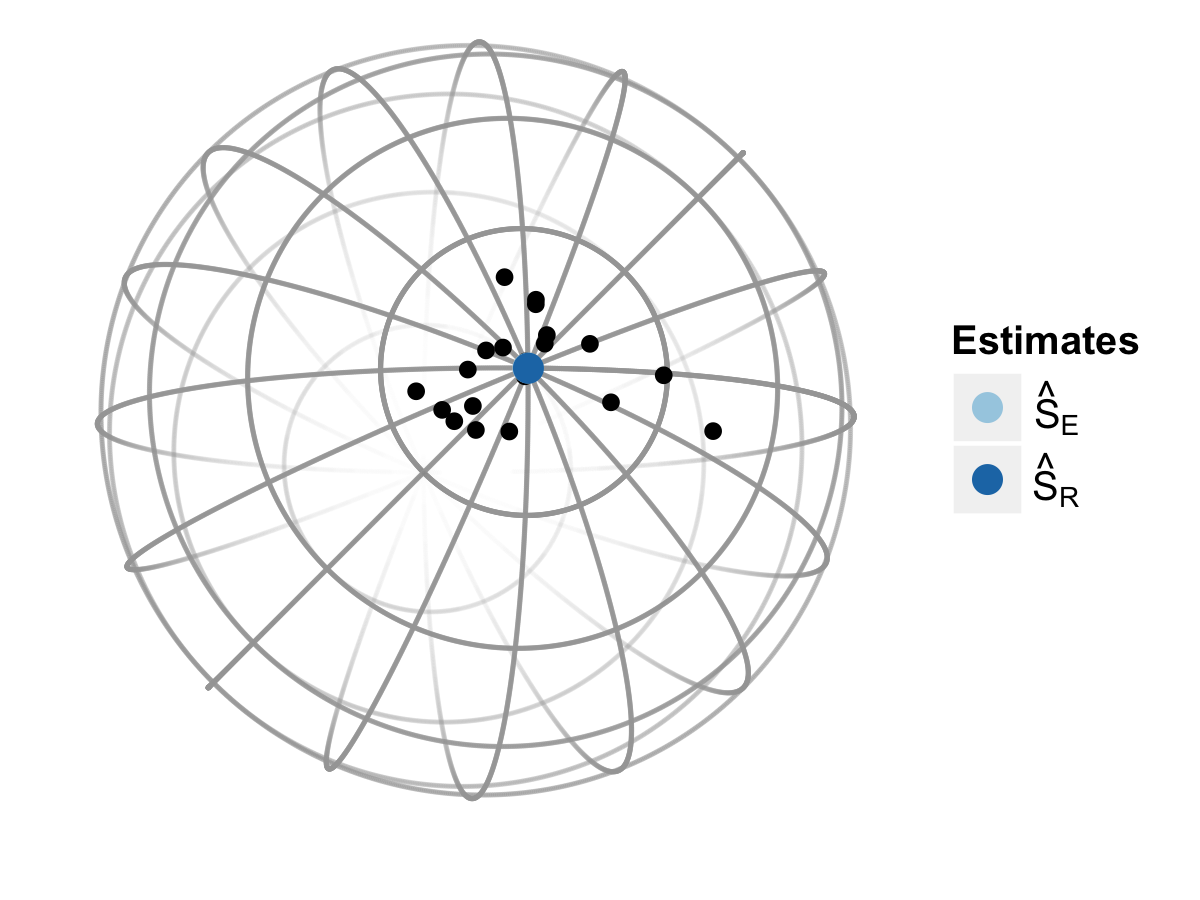
\includegraphics[width=\textwidth]{Figure/Sample1}
  \caption{Original data, A}
  \label{fig:samp1}
\end{subfigure}
\begin{subfigure}[b]{0.45\textwidth}
  \centering
  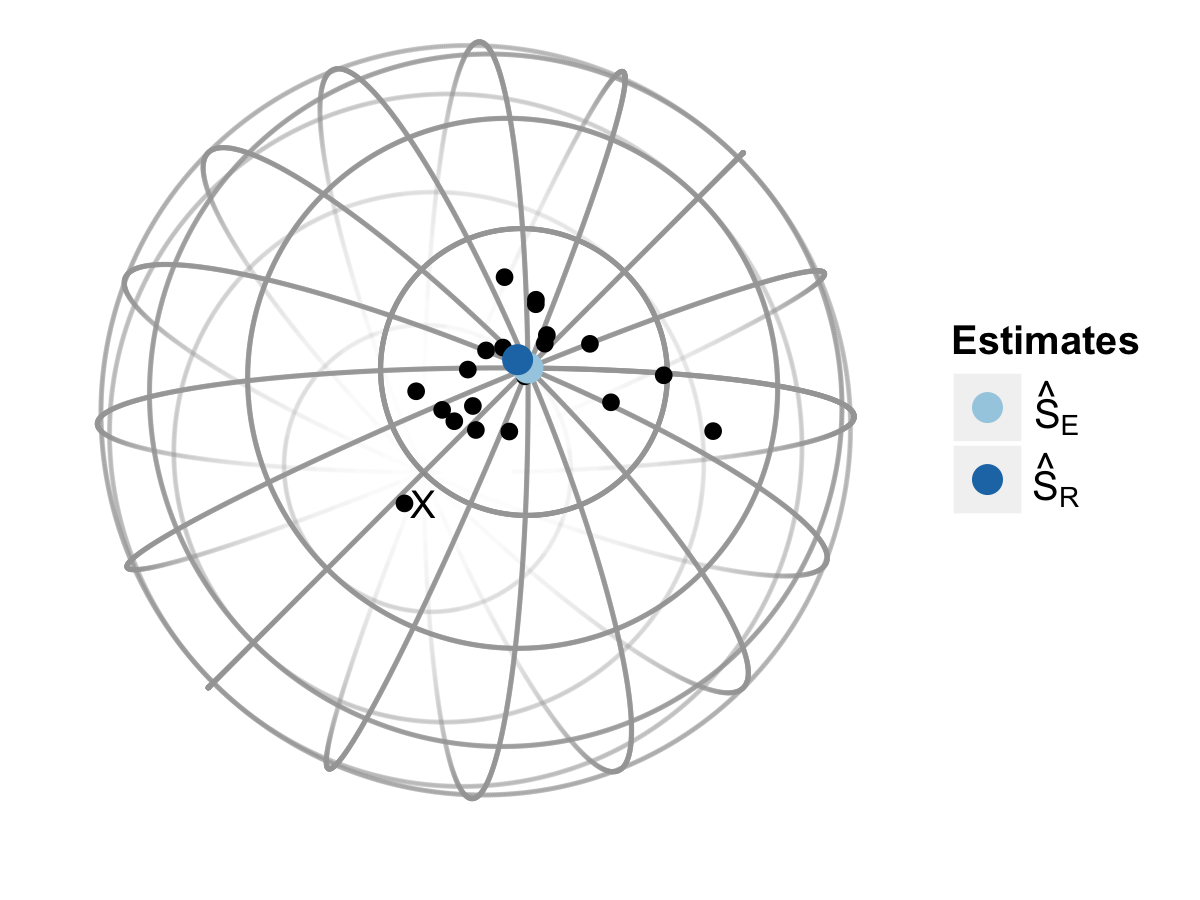
\includegraphics[width=\textwidth]{Figure/Sample2}
  \caption{Altered data, B}
  \label{fig:samp2}
\end{subfigure}
\caption{Random sample of size $20$ from Cayley($\bm I_{3\times 3},50$) distribution in (a).  Same sample with additional observation that is the rotation of $\ProjMean$ rotated through 180$^\circ$ about an arbitrary axis in (b), marked with an ``X".  Notice $\ProjMean$ is exactly the same in both samples, but $\GeomMean$ moves away.}
\label{fig:sample}
\end{figure}
\clearpage
\section{Robustified Means}

In this section I use the $H_i$ and $C_i$ statistics to robustify the projected $\ProjMean$ $L_2$ estimator.  In particular I look at the trimmed, weighted and winsorized mean as well as the Huber estimator.  I think it would be simple to extend these ideas to the geometric $L_2$ estimator $\GeomMean$.

To define the $SO(3)$ \emph{trimmed mean} we need to determine which observations are in the tails.  To do this consider the the discordant measure $H_i$ proposed by \cite{best1986} and later expanded to the hypersphere by \cite{figueiredo2005} defined in Section \ref{sec:outliers}.

It follows that $\alpha$-trimmed mean in $SO(3)$ is defined by
\[
\bm S_{T}=\int_{SO(3)}\bm Rf^*(\bm R|\bm S,\kappa)d\bm R
\]
where $f^*(\bm R|\bm S,\kappa)$ is the rotational distribution that puts $0$ probability on rotations $\bm R_i$ with $H_i$ statistics beyond the $100(1-\alpha)\%$ of the $H_i$ distribution.  In practice $\bm S_T$ can be estimated by
\[
\TrimMean=\argmax_{\bm S\in SO(3)}\text{tr}(\bm S^\top\overline{\bm R}_T)
\]
where $\overline{\bm R}_T=\sum_{i=1}^n\bm R_iI( H_i\leq \hat H_\alpha)$ and $\hat H_{\alpha}$ is the $100(1-\alpha)\%$ of the distribution of $H_i$.


Define the $SO(3)$ \emph{weighted mean} as
\begin{align*}
\WeightMean=\argmax_{\bm S\in SO(3)}\text{tr}(\bm S^\top\overline{\bm R}_W)
\end{align*}
where $\overline{\bm R}_W=(\sum_{i}w_i\bm R_i)/(\sum_i w_i)$, the weights $w_i^{-1}=\sqrt{H_i}/(\sum_i \sqrt{H_i})$ and $H_i$ is from \eqref{eqn:Hj}.  I use the square root of $H_i$ because $H_i$ alone behaves like a square loss function instead of an absolute loss function.


The idea of the multidimensional \emph{Huber estimator} is to robustify an estimator by placing a bound on the norm of its influence function.  In Figure \ref{fig:Huber} the 2-dimensional case is illustrated for the artificial data $\bm R_1,\dots,\bm R_6$.
\begin{figure}[h]
\begin{center}
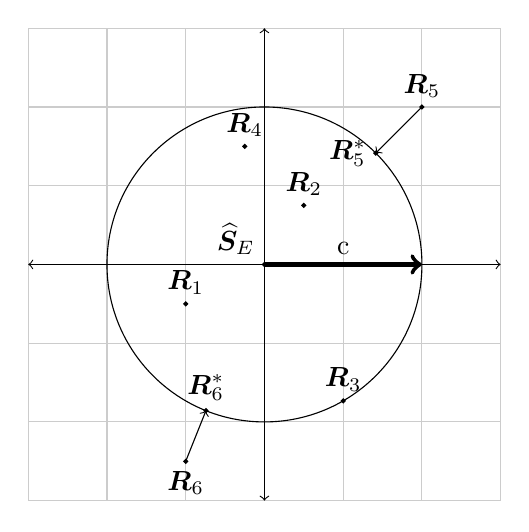
\begin{tikzpicture}
    \draw [black!20] (-3,-3) grid (3,3);
    \draw (0,0) circle [radius=2];
    \draw [->,ultra thick] (0,0) -- (2,0);
    \draw [<->] (-3,0) -- (3,0);
    \draw [<->] (0,-3) -- (0,3);
    \node [above left] at (0,0) {$\widehat{\bm S}_E$};
    \draw [fill] (0,0) circle [radius=0.025];
    \node [above] at (1,0) {c};
    \node [above] at (-1,-.5) {$\bm{R}_1$};
    \draw [fill] (-1,-.5) circle [radius=0.025];
    \node [above] at (.5,.75) {$\bm{R}_2$};
    \draw [fill] (.5,.75) circle [radius=0.025];
    \node [above] at (1,-1.732051) {$\bm{R}_3$};
    \draw [fill] (1,-1.732051) circle [radius=0.025];
    \node [above] at (-.25,1.5) {$\bm{R}_4$};
    \draw [fill] (-.25,1.5) circle [radius=0.025];
    \node [above] at (2,2) {$\bm{R}_5$};
    \draw [fill] (2,2) circle [radius=0.025];
    \node [left] at (1.414214, 1.414214) {$\bm{R}_5^*$};
    \draw [fill] (1.414214, 1.414214) circle [radius=0.025];
    \draw [->] (2,2) -- (1.414214, 1.414214);
    \node [below] at (-1,-2.5) {$\bm{R}_6$};
    \draw [fill] (-1,-2.5) circle [radius=0.025];
    \node [above] at (-0.7427814,  -1.8569534) {$\bm{R}_6^*$};
    \draw [fill] (-0.7427814, -1.8569534) circle [radius=0.025];
    \draw [->] (-1,-2.5) -- (-0.7427814,  -1.8569534);
\end{tikzpicture}
\end{center}
\caption{Multidimensional Huber estimator with estimated center $\ProjMean$ as illustrated in Section 4.3 of \cite{hampel2011}.}
\label{fig:Huber}
\end{figure}

Each point represents the influence function evaluated at that data point.  The norm of the influence function for this estimator evaluated at $\bm R_1,\dots,\bm R_4$ all lie within the specified range of the estimated center so they are left untouched.  The norm of the influence function evaluated at $\bm R_5$ and $\bm R_6$ however is larger than $c$ and therefore those points are altered such that the norm of the influence function has a norm of $c$.  The reason (according to page 239 of \citealt{hampel2011}) for placing the bound on the influence function is because  ``the most meaningful version of the $\psi$-function defining an $M$-estimator is its influence function."

Applying this idea to $SO(3)$ data, recall from \eqref{eqn:IF} that $\text{IF}\propto\sin(r)\bm U_i$ where $\bm U_i$ has norm one, thus $\|\text{IF}(\bm R_i,F)\|\propto \sin(|r|)$.  It follows that using the Huber estimator directly will put the most restrictions on the rotations $\bm R_i$ that are near $\pi/2$ radians away from the estimated center instead of observations as far as $\pi$ radians away.  Alternatively a modified Huber estimator on $SO(3)$ could puts a bound on $\hat r_i=d_r(\bm R_i,\ProjMean)$.  

The algorithm I use to compute $\HuberMean$ based on the sample $\bm R_1,\dots,\bm R_n$ and the constant $c$ is as follows
\begin{enumerate} 
\item Compute $\ProjMean^{(j)}$
\item For each $i$ compute $\hat r_i^{(j)}=d_r(\bm R_i,\ProjMean^{(j)})$
\item For each $i$ such that $r_i>c$:
\begin{enumerate}
\item Find $\bm u_i\in\mathcal{S}^3$ satisfying $\exp[\bm{\Phi}(r_i\bm u_i)]=\ProjMean^{(j)\top}\bm R_i$
\item Redefine $\bm R_i=\ProjMean^{(j)\top}\exp[\bm{\Phi}(c\bm u_i)]$
\end{enumerate}
\item Repeat steps 1 - 3 for $j+1$ until $r_i<c$ for all $i$
\item Define $\HuberMean=\ProjMean^{(j+1)}$
\end{enumerate}
Figure \ref{fig:huberContd} illustrates the modified Huber estimator for a variety of $c$ values.  Notice that when the $c$ value is very small, then the data converge quickly to the initial estimate of center, which is the opposite of what we would like to do.

% \begin{figure}[h]
% \begin{center}
% \animategraphics[width=.5\textwidth,controls,loop]{1}{Figure/huberContd}{1}{11}
% \end{center}
% \caption{The modified Huber estimator (limit the distance from the estimated central direction) for a range of c values.}
% \label{fig:huberContd}
% \end{figure}

An $SO(3)$ interpretation of the \emph{winsorized mean} is a combination of the $SO(3)$ trimmed mean and modified Huber estimator.  That is, the data are ordered according to their statistic values, e.g.~$H_i$ or $C_I$.  All rotations beyond the upper $100(1-\alpha)$\% percentage of that statistic is projected to the border of the inner circle while maintaining the original axis of rotation.  The mathematical definition is 
\[
\WinzMean=\argmax_{\bm S\in SO(3)}\text{tr}(\bm S^\top\overline{\bm R}_{Z})
\]
where $\overline{\bm R}_{Z}=\sum_{i=1}^n\bm R_i^*/n$, 
\[
\bm R_i^*=
\begin{cases}
\bm R_i&\text{ if }d_R(\ProjMean,\bm R_i)\leq\hat{q}\\
\ProjMean\exp[\bm{\Phi}(\hat{q}\bm{u}_i^*)]&\text{ otherwise,}
\end{cases}
\]
$\bm U_i^*$ is the axis of rotation corresponding to $\ProjMean^\top\bm R_i$ and $\hat{H}_\alpha$ is the $100(1-\alpha)$\% percentile of the distribution of $H_i$.




\section{(Very) Limited Simulation Study}

Below is a a very small simulation study comparing the usual estimators and two versions of each robustified $L_2$ estimator (trimmed, winsorized, weighted, Huber).  The two versions of robustification come from the choice of statistics to determine ``outliers": either $H_i$ which identifies observations far from the bulk of the data (Tables \ref{tab:SimResHn} and \ref{tab:SimResHnIntrin}), or $C_i$ which identifies observations that influence the estimated center (Table \ref{tab:SimResC}).  One-hundred samples per combination of distribution (Cayley or von Mises Fisher), sample size ($n=10,50$), concentration ($\kappa=0.5,1,10$) all with $10\%$ contamination.  That is 90\% of the final data set comes from the respective $F(\bm I_{3\times 3},\kappa)$ distribution and the remaining 10\% of the sample comes from a $F(\bm S_c[\pi/2,\bm u],\kappa)$.  In the circular/spherical data set this is called the slippage alternative.  

Tables \ref{tab:SimResHn} and \ref{tab:SimResC} include results for the extrinsic mean $\ProjMean$ and median $\ProjMedian$. Both methods to identify extreme observations are used because of the results of Section \ref{sec:outliers}.  Table \ref{tab:SimResHnIntrin} includes results for the intrinsic mean $\GeomMean$ and median $\GeomMedian$ with robustified versions of $\GeomMean$ based on $H_i$ statistic since it is linearly related to $C_i$, again from the results of Section \ref{sec:outliers}.

In Table \ref{tab:SimResHn} is the average bias based on the Euclidean distance in each estimator for each simulated scenario.  That is bias$=\|\bm I_{3\times 3}-\widehat{\bm S}\|_F$ for each estimator.  The trimmed and winsorized mean use $\alpha=0.1$ and the Huber estimator sets $c=0.75$.


\begin{table}[ht]
\centering
\begin{tabular}{l|lll|lll|lll|lll}
  \hline
 & \multicolumn{6}{|c|}{Cayley} & \multicolumn{6}{|c}{von Mises}   \\ 
\hline
   &  \multicolumn{3}{|c|}{n=10} & \multicolumn{3}{|c|}{n=50} & \multicolumn{3}{|c|}{n=10} & \multicolumn{3}{|c}{n=50} \\ 
  $\kappa$ &  0.5 &  1.0 & 10.0 &  0.5 &  1.0 & 10.0 &  0.5 &  1.0 & 10.0 &  0.5 &  1.0 & 10.0 \\ \hline
  $\ProjMedian$ (Median) & 1.71 & 1.30 & 0.37 & 0.92 & 0.66 & 0.18 & \red{0.52 }& \red{0.33} & \red{0.09} & \red{0.15} & \red{ 0.11} & \red{ 0.03} \\ 
  $\ProjMean$ (Mean) & \red{1.55} & \red{1.10} & 0.35 & 0.79 & 0.55 & 0.21 & 0.66 & 0.49 & 0.20 & 0.31 & 0.23 & 0.17 \\ 
  $\TrimMean$ (Trim) & 1.56 & 1.16 & \red{0.34} & 0.80 & 0.57 & \red{0.16} & 0.70 & 0.52 & 0.13 & 0.33 & 0.24 & 0.06 \\ 
  $\WinzMean$ (Winsorize)& 1.56 & 1.11 & 0.36 & \red{0.75} & \red{0.51} & 0.21 & 0.68 & 0.51 & 0.18 & 0.32& 0.24 & 0.12 \\ 
  $\WeightMean$ (Weight) & 1.60 & 1.17 & 0.41 & 0.83 & 0.63 & 0.19 & 0.56 & 0.39 & 0.11 & 0.19 & 0.16 & 0.08 \\ 
  $\HuberMean$ (Huber) & \red{1.55} & 1.11 & 0.35 & 0.77 & 0.54 & 0.20 & 0.65 & 0.47 & 0.17 & 0.30 & 0.22 & 0.13 \\ 
   \hline
\end{tabular}
\caption{Mean estimator bias based on 100 samples from each combination of distribution, sample size and concentration.  The projected $L_2$ estimator $\ProjMean$ is robustified based on the ordering of the data determined by $H_i$ statistic (i.e.~distance from the bulk of the data).}
\label{tab:SimResHn}
\end{table}

Results when the $H_i$ statistic is used to robustify $\ProjMean$ are in Table \ref{tab:SimResHn}.  For the Cayley (and presumably Fisher matrix) distribution, the traditional mean, Huber estimator and trimmed mean are close.  Trimmed mean is preferred for more concentrated data and the Huber estimator is preferred as the data become less concentrated.  A possible explanation is that the trimmed mean is discarding the contaminated data when the bulk of the data is highly concentrated, while the Huber estimator is trying to use all the data.  As was demonstrated in the Technometric paper, the median does really poorly.

For the von Mises distribution in Table \ref{tab:SimResHn}, it looks like the median is unbeatable.  This is likely due to the heavy tail we identified in the Technometrics paper.  Similar to the other distribution, the trimmed mean improves considerably as the bulk of the data becomes more concentrated and the contamination can be cut out completely.  The Huber estimator and winsorized mean give comparable results but are great.

\begin{table}[ht]
\centering
\begin{tabular}{l|lll|lll|lll|lll}
  \hline
 & \multicolumn{6}{|c|}{Cayley} & \multicolumn{6}{|c}{von Mises}   \\ 
\hline
   &  \multicolumn{3}{|c|}{n=10} & \multicolumn{3}{|c|}{n=50} & \multicolumn{3}{|c|}{n=10} & \multicolumn{3}{|c}{n=50} \\
  $\kappa$ &  0.5 &  1.0 & 10.0 &  0.5 &  1.0 & 10.0 &  0.5 &  1.0 & 10.0 &  0.5 &  1.0 & 10.0 \\ \hline
  $\ProjMedian$ (Median) & 1.70 & 1.25 & 0.35 & 1.01 & 0.59 & 0.19 & \red{ 0.55} & \red{ 0.37}& \red{ 0.08} & \red{ 0.15} & \red{ 0.11} & \red{ 0.03} \\ 
  $\ProjMean$ (Mean) & \red{ 1.56} & 1.04 & \red{ 0.33} & 0.83 & 0.49 & 0.22 & 0.76 & 0.50 & 0.19 & 0.30 & 0.25 & 0.17 \\ 
   $\TrimMean$ (Trim) & 1.68 & 1.12 & 0.34 & 0.86 & 0.52 & \red{ 0.17} & 0.82 & 0.53 & 0.13 & 0.31 & 0.23 & 0.06 \\ 
  $\WinzMean$ (Winsorize) & 1.60 & 1.06 & 0.34 & \red{ 0.82} & 0.49 & 0.18 & 0.74 & 0.51 & 0.13 & 0.29 & 0.22 & 0.06 \\ 
  $\WeightMean$ (Weight) & 2.07 & 1.52 & \red{ 0.33} & 2.06 & 0.83 & 0.20 & 1.37 & 0.74 & 0.12 & 0.75 & 0.41 & 0.08 \\ 
  $\HuberMean$ (Huber) & \red{ 1.56 }& \red{ 1.03} & \red{ 0.33} & \red{ 0.82} & \red{ 0.48} & 0.20 & 0.74 & 0.49 & 0.16 & 0.28 & 0.23 & 0.13 \\ 
   \hline
\end{tabular}
\caption{Mean estimator bias based on 100 samples from each combination of distribution, sample size and concentration.  The projected $L_2$ estimator $\ProjMean$ is robustified based on the affect each observation has on $\ProjMean$ as determined by $C_i$ statistic (i.e.~empirical influence function).}
\label{tab:SimResC}
\end{table}

The results in Table \ref{tab:SimResC} include results for when robustification is based on the influence function or the affect each observation has on the estimate of center.  For this case the Huber estimator does well for the Cayley distribution.  The trimmed mean does well when the data become highly concentrated and that is likely due to the same reason as before.  Again the median is best for the von Mises Fisher distribution.  

Also of note in Table \ref{tab:SimResC} is how terrible the weighted mean $\WeightMean$ does in a majority of the situations.  This is likely due to the fact that the $C_i$ statistic will put weight on observations far from the estimated center, so long as they are not near $\pi/2$ radians away from that estimate.  This could result putting a lot of weight on an observation that could draw the estimate far off course.

Finally in Table \ref{tab:SimResHnIntrin} are results for the intrinsic mean/median along with the robustified intrinsic mean. Similar to the results for the Cayley distribution in Tables \ref{tab:SimResHn} and \ref{tab:SimResC} the mean is generally preferred to the other estimators; unlike the earlier results, however, the trimmed mean performs well especially for concentrated data.  For the von Mises distribution the geometric median is preferred, which is to be expected.  Unexpected is how well the weighted mean is doing.  I suspect the Huber estimator will perform better when the $c$ value is chosen appropriately, not arbitrarily (as was done here).

\begin{table}[ht]
\centering
\begin{tabular}{l|lll|lll|lll|lll}
  \hline
 & \multicolumn{6}{|c|}{Cayley} & \multicolumn{6}{|c}{von Mises}   \\ 
\hline
   &  \multicolumn{3}{|c|}{n=10} & \multicolumn{3}{|c|}{n=50} & \multicolumn{3}{|c|}{n=10} & \multicolumn{3}{|c}{n=50} \\
  $\kappa$ &  0.5 &  1.0 & 10.0 &  0.5 &  1.0 & 10.0 &  0.5 &  1.0 & 10.0 &  0.5 &  1.0 & 10.0 \\ \hline
 $\GeomMedian$ (Median) & 1.57 & 1.06 & 0.37 & 0.77 & 0.49 & 0.19 & 0.60 & 0.39 & \red{0.09} & \red{0.18} & \red{0.15} & \red{0.04} \\ 
 $\GeomMean$ (Mean) & \red{1.54} & \red{0.99} & 0.40 & \red{0.68} & \red{0.43} & 0.24 & 0.92 & 0.64 & 0.25 & 0.44 & 0.37 & 0.23 \\ 
 $\TrimMean$ (Trim) & \red{1.54} & \red{0.99} & \red{0.34} & 0.73 & 0.45 & \red{0.16} & 0.93 & 0.66 & 0.14 & 0.44 & 0.38 & 0.07 \\ 
 $\WinzMean$ (Winsorize) & \red{1.54} & 1.00 & 0.40 & 0.71 & 0.45 & 0.28 & 0.87 & 0.68 & 0.22 & 0.43 & 0.37 & 0.33 \\ 
 $\WeightMean$ (Weight) & 1.60 & 1.09 & 0.38 & 0.86 & 0.55 & 0.20 & \red{0.57} & \red{0.38} & 0.11 & \red{0.18} & 0.16 & 0.08 \\ 
 $\HuberMean$ (Huber) & 1.55 & 1.01 & 0.36 & 0.70 & 0.45 & 0.19 & 0.80 & 0.53 & 0.17 & 0.35 & 0.29 & 0.13 \\ 
   \hline
\end{tabular}
\caption{Mean estimator bias based on 100 samples from each combination of distribution, sample size and concentration.  The geometric $L_2$ estimator $\GeomMean$ is robustified based on the ordering of the data determined by $H_i$ statistic (i.e.~distance from the bulk of the data).}
\label{tab:SimResHnIntrin}
\end{table}

% \begin{figure}
% \centering
% 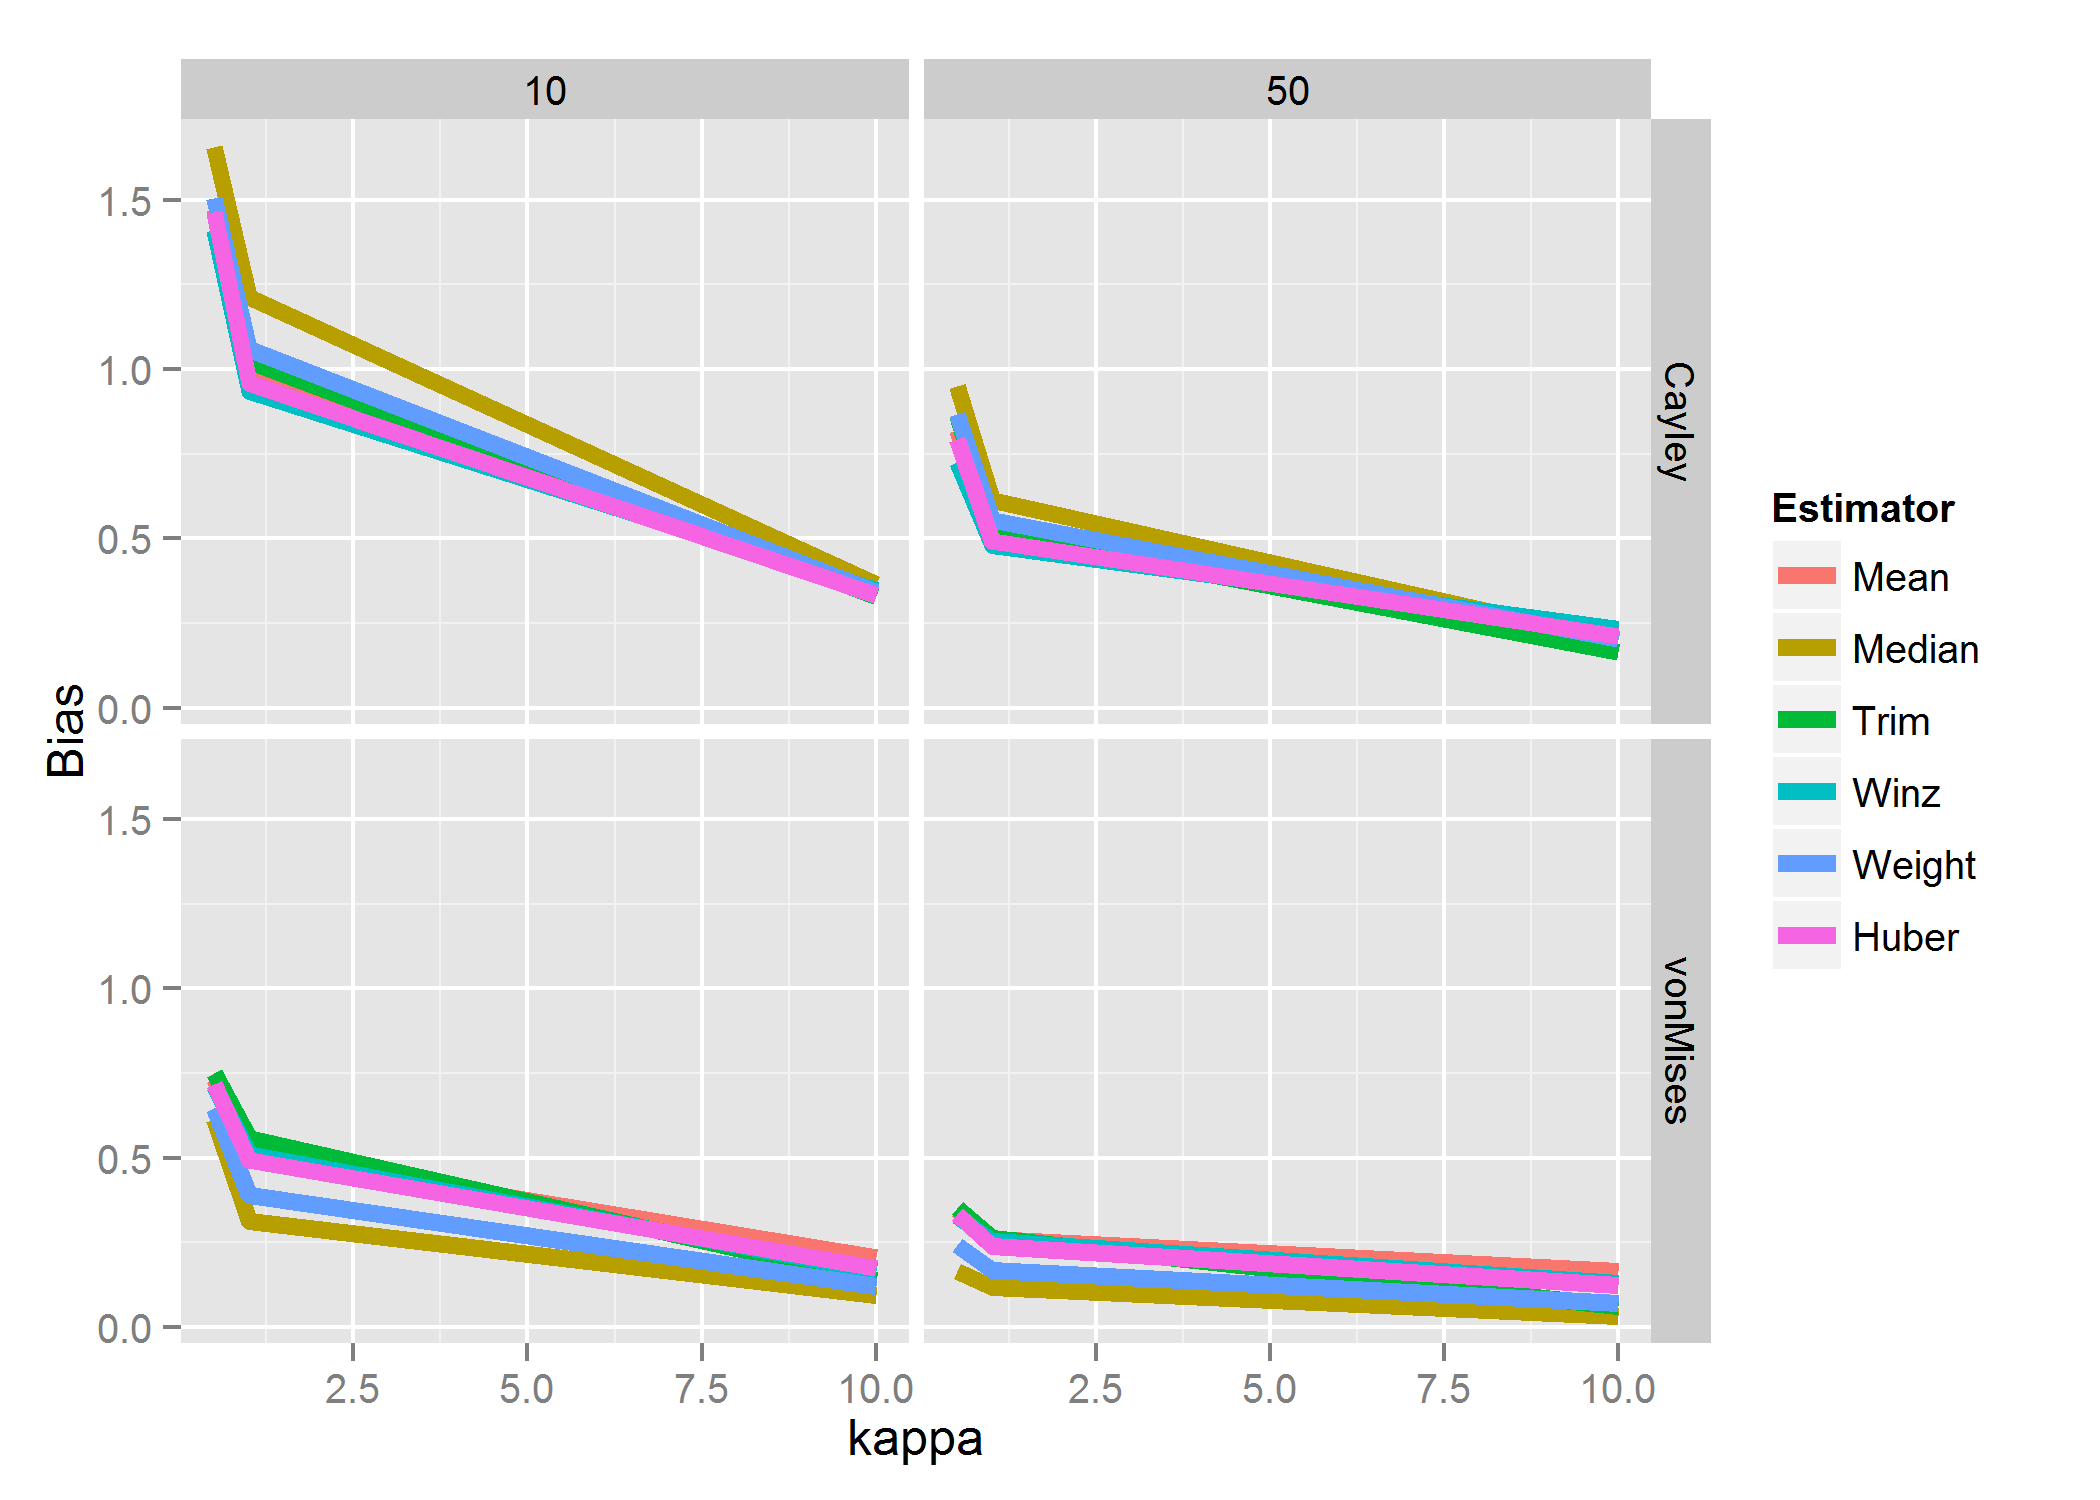
\includegraphics[width=.7\textwidth]{Estimator.png}
% \caption{Graphical representation of Table \ref{tab:SimResHn} faceted by sample size and distribution.}
% \end{figure}



\clearpage
%\bibliographystyle{plain}
\bibliography{../OutlierDetection/RobustRefs}
\end{document}
